\section{Literature Conversions for Figure~\ref{fig:heateffects}}
\label{app:conversions}

Published heat effects are reported in incompatible units, and Figure~\ref{fig:heateffects} places them
on one axis. The conversions are as follows. Slopes given in seconds per degree are divided by a
representative finish time for the population studied, 130 minutes for elite fields and 240 minutes
for mass fields, giving a percentage per degree. Effects reported as a percentage over an interval,
such as a change per 5\,\textdegree C, are divided by the interval width. All curves are anchored at
10\,\textdegree C, so each shows slowdown relative to that reference rather than an absolute time.

Two limitations apply. Studies native to air temperature are drawn on the same axis as studies native
to WBGT, which are not interchangeable: the offset between them depends on humidity, radiation and
wind, so placement above roughly 18\,\textdegree C is approximate. And the published quadratics are
drawn only across the range over which they were fitted. A quadratic with a positive second-order
term diverges outside its support, and extrapolating one of the fitted clusters to 28\,\textdegree C
would imply a slowdown near 50\%, which is an artifact of the functional form rather than a claim
made by its authors.

% ===========================================================================
% tommy_appendix.tex -- the biophysical account of why the heat penalty is
% convex. Kept in its own file so it can be edited without conflicting with
% appendix.tex. It owns \label{app:physics}, which the main text references
% twice.
%
% NOTE: an Overleaf round-trip moved "Literature Conversions for Figure 4"
% (Appendix E) out of appendix.tex and into the TOP of this file. It renders in
% the same place either way, since appendix.tex is \input immediately before
% this one, so it has been left where it is -- but this file now carries two
% unrelated appendices, and E must stay above the \section below.
%
% Every number here is reproduced by verify_heat_convexity.py (stdlib only,
% self-checking, prints ok/FAIL per line, currently ALL CHECKS PASSED). The
% four figures are built by build_compensability_figures.py.
%
% Structure of the argument, so an editor can see the spine at a glance:
%
%   F.1  Heat balance at steady state is one equation in one unknown, the
%        runner's speed. That is why pace is the variable that gives.
%   F.2  The whole environment enters through one scalar, the thermal head
%        Phi, which is decreasing and CONCAVE in wet-bulb temperature.
%   F.3  A concave speed limit makes a convex pace penalty. Theorem, not a
%        parameter sweep. But the hard ceiling binds only in the mid-20s.
%   F.4  So the response below the ceiling is graded, and w_req -- the
%        wettedness measure -- is convex for the same Clausius-Clapeyron
%        reason. The wettedness result is a corollary, not a separate fact.
%   F.5  The same balance read as a demand on cardiac output, which carries
%        the same curvature. Not a rival account; the next link in the chain,
%        sharing the boundary T_sk, which is why T_sk dominates everything.
%   F.6  Duration. The storage allowance B = m*c*dT is a FIXED quantity of
%        heat, so the distance it covers, d_bank = B/kappa ~ 2.6 km, is
%        independent of both pace and body mass (both cancel). Heat cannot
%        bind a race shorter than that, which is the sprint/marathon split.
%   F.7  The measured curvature.  F.8  The dry-bulb axis.
%   F.9  What this does and does not establish.
%
% The preamble carries a roadmap of the above, added deliberately: the chain
% (surface link -> transport link, coupled through T_sk) was previously only
% visible to a reader who had already got as far as F.5.
%
% REQUIRES THREE EDITS ELSEWHERE IN THE MANUSCRIPT (see handoff notes):
%  * Section 2 currently uses T_sk = 35 C and says dry exchange reverses "near
%    36 C". Adopting 31 C moves the reversal to 31 C and changes the 83/14/4
%    evaporation shares. These must agree or a referee will catch it.
%  * Appendix C's isopleth table (\label{tab:isopleth}) is computed at
%    T_sk = 35 C, total 873.5. Table \ref{tab:wbtradeoff} below supersedes it at
%    T_sk = 31 C, total 555.1, so DELETE the appendix one rather than keeping
%    two isopleths at different skin temperatures. The labels differ, so
%    nothing breaks if you leave it in place -- it will just contradict.
%  * Appendix C reports the learned steepening as 2.12; this insert uses 2.18.
%    Settle which is current.
% ===========================================================================

% Kept at \section level deliberately. The Overleaf round-trip demoted this to
% \subsection and dropped \label{app:physics}, which had two consequences: the
% main text's two "Appendix~\ref{app:physics}" pointers rendered as "??", and
% the whole biophysical account nested underneath "Literature Conversions for
% Figure 4" as E.1-E.10, since that section now opens this same file. The title
% below is left exactly as the Overleaf edit set it. \label{sec:convexity} is
% preserved as an alias so nothing added against it dangles; nothing references
% it at present.
\section{Why the penalty accelerates: a biophysical account}
\label{app:physics}
\label{sec:convexity}

This appendix supports the physical argument in Section~\ref{sec:results}. It
makes one claim in several places: the acceleration in the measured heat
penalty is not a fitted shape but a consequence of the heat balance, and it
traces to a single term, the curvature of saturation vapour pressure with
temperature. Everything else in the calculation moves the size of the effect
without touching its shape.

The argument runs in one direction, and it is worth having the whole of it in
view before the algebra starts. A runner at the limit of effort has no lever
left but pace: metabolic heat production is fixed by speed, the external work
term is not free to move, and once core temperature has stopped rising the heat
balance ceases to be an accounting identity and becomes an equation in the
single unknown $v$ (Section~\ref{app:physics:limit}). Heat is governed by speed
and speed by heat, in other words, only because the runner is already at
maximum metabolic rate; a runner with something in reserve is not on this
constraint at all. What the environment will accept on the other side of that
equation then turns out to depend on one number rather than two, a
\emph{thermal head} that collapses air temperature and humidity into a single
quantity carried in kelvin-equivalents (Section~\ref{app:physics:head}). That
head does two things. It falls as conditions warm, and it falls at an
accelerating rate, because saturation vapour pressure is convex in temperature.
So the dissipation ceiling, and the speed it permits, are decreasing and
\emph{concave} in wet-bulb temperature. A pace penalty is a reciprocal of a
permitted speed, and the reciprocal of a decaying concave function is convex
(Section~\ref{app:physics:convex}). That is the whole of the result, and it is
a theorem about the heat balance rather than a curve fitted to our data.

The hard ceiling binds only in the mid-twenties, while the measured curve bends
near $16\,^{\circ}$C, so runners are evidently responding to something graded
well below the point at which balance fails. That something is \emph{required
wettedness}: the evaporation the balance demands divided by the maximum the air
will accept, or equivalently the fraction of the skin that must be covered in
sweat to hold pace. It is a ratio of demand to capacity rather than a measure
of effort, it can be read at any condition rather than only at the limit, and
it inherits the same denominator, so it is convex in wet-bulb temperature for
the same one reason (Section~\ref{app:physics:graded}).

Wettedness is a statement about the skin, and it says nothing about how the
heat reached the skin. That is a second constraint, and the two are consecutive
links in one chain rather than competing accounts. Heat is made in muscle and
can only be carried to the surface by blood, so the same balance can be written
as a required skin blood flow, which is a claim on cardiac output
(Section~\ref{app:physics:circulation}). The links share a boundary, mean skin
temperature, and they pull on it in opposite directions: warmer skin widens the
skin-to-air gradients and eases the surface link, while narrowing the
core-to-skin gradient and tightening the transport link hyperbolically. They
are loaded twice over by the same sweat, since the fluid that evaporates at the
surface leaves the circulation to do it, which is the cost the last column of
Table~\ref{tab:wbtradeoff} prices. Both links carry the same curvature, and
they must, so the convexity appears whichever one is measured. How much of a
transient imbalance a runner may simply ignore is then a question of how long
they must ignore it for, which is why heat governs a marathon and barely
touches a mile (Section~\ref{app:physics:duration}).

The three closing sections test the account rather than extend it: against the
curvature actually measured (Section~\ref{app:physics:curvature}), on the
thermometer's own axis, where it makes its sharpest and most falsifiable
prediction (Section~\ref{app:physics:drybulb}), and against the competing
explanations and statistical artifacts it cannot rule out
(Section~\ref{app:physics:limits}).

All coefficients are those reported by \citet{taylor2006} and already used in
Section~\ref{sec:literature}: convective exchange $8.3\,(T_{sk}-T_a)\sqrt{v}$,
radiant $5.2\,(T_{sk}-T_{mrt})$ and evaporative $124\,(P_{sk}-P_a)\sqrt{v}$ per
square metre. Calculations assume a $70\,\mathrm{kg}$ runner with
$1.85\,\mathrm{m^2}$ of body surface at three-and-a-half-hour marathon speed,
$3.33\,\mathrm{m\,s^{-1}}$, producing $770\,\mathrm{W}$ of heat, or
$416\,\mathrm{W\,m^{-2}}$.

Mean skin temperature is taken as $31\,^{\circ}$C rather than the
$35\,^{\circ}$C typical of laboratory treadmill work. \citet{aylwin2023}
measured it falling from $29.8$ to $28.9\,^{\circ}$C through the men's marathon
at the 2019 World Championships, below air temperature, because airflow at
running speed cools wet skin. As shown in Section~\ref{app:physics:curvature},
this is the single most consequential input in the calculation, and the
paragraph above says why: skin temperature is the boundary the two links share,
so it enters the surface balance and the transport balance at once.

\subsection{The heat balance is a speed limit}
\label{app:physics:limit}

Section~\ref{sec:literature} gives heat balance as an accounting identity,
\begin{equation}
  S \;=\; M \;-\; W \;-\; (R + C + K) \;-\; E,
  \label{eq:balance}
\end{equation}
with $S$ the rate of heat storage in body tissue, $M$ metabolic heat
production, $W$ the external mechanical work leaving the body, and $R$, $C$,
$K$ and $E$ the radiative, convective, conductive and evaporative exchanges.
Written this way it is a bookkeeping statement. It becomes a statement about
pace once one notices which of its terms a runner actually controls.

Only one. Running economy is close to constant in energy per unit distance
rather than per unit time, so metabolic rate is proportional to speed,
$M \approx c\,m\,v$ with $c$ near $4.2\,\mathrm{kJ\,kg^{-1}\,km^{-1}}$. The
work term is not an independent lever either: at a given speed the mechanical
work of running is fixed by the mechanics of running at that speed. A runner
in difficulty cannot buy thermal relief by doing less external work while
holding pace. Taking the conventional $20$ to $25\%$ of turnover as work,
production and work both scale with $v$, and so does their difference,
\begin{equation}
  H \;=\; M - W \;=\; \kappa\,v, \qquad
  \kappa \;\approx\; 231\,\mathrm{J\,m^{-1}}
  \label{eq:production}
\end{equation}
for the reference runner. Two remarks on $\kappa$.

It is conservative, and the reason is worth stating because the work term is
where a heat balance for running differs from one for cycling. In level
locomotion there is no external force adding positive power to the runner: the
ground reaction force is applied at a point with zero velocity, so the
propulsive product vanishes identically and gross efficiency \emph{against the
environment} is close to zero rather than close to a quarter
\citep{vaningenschenau1990}. ISO 7933 accordingly sets $W = 0$ outright for
this reason \citep{iso7933}. What genuinely leaves the system is the work
against air resistance, about $2\%$ of metabolic cost at marathon speed
\citep{davies1980} and, once that cost is multiplied by efficiency to give
work, well under one percent. Equation~\eqref{eq:production} therefore charges
the runner less heat than the physics does, not more.\footnote{This is a claim
about work done on the \emph{environment}, which is the thermodynamically
relevant quantity. It should not be confused with the separate observation that
positive and negative work on the centre of mass cancel over a stride: that
cancellation is a bookkeeping identity and does not by itself establish that
any energy left the body.}

The second remark is that nothing below turns on a drift in $\kappa$ with
conditions, which is fortunate, because the effect of heat stress on running
economy is equivocal in the literature; \citet{james2017} report it slightly
\emph{improved} in the heat.

Now impose the two conditions that describe a runner racing. The first is that
effort is already maximal, so the runner is not holding anything back. The
second is that heat storage has stopped, $S = 0$: core temperature is no
longer rising, either because the runner has reached the ceiling they can
tolerate or because the race is long enough that a sustained imbalance is not
available. Under those two conditions \eqref{eq:balance} loses its slack and
becomes an equation in the single unknown $v$,
\begin{equation}
  \kappa\,v \;=\; R + C + E .
  \label{eq:pinned}
\end{equation}
This is the sense in which heat sets a speed limit. The right-hand side is what
the environment will accept, and it does not care how much the runner wants to
run. If the runner's chosen $v$ makes the left-hand side larger, the equality
fails in the only way it can, through $S > 0$: core temperature climbs. That is
survivable, but only for a while and only by a bounded amount, which is why the
constraint tightens with race duration (Section~\ref{app:physics:duration}). Once the
tolerable rise is spent, balance must be restored, and the only term left to
move is $v$. The runner slows.

\subsection{The environment enters through a single number}
\label{app:physics:head}

Write the right-hand side of \eqref{eq:pinned} at its maximum. With skin fully
wetted, the capacity to shed heat is the sum of a dry and an evaporative term,
\begin{equation}
  Q_{\max} = h_c\,(T_{sk} - T_a) \;+\; h_e\,\bigl(P_{s}(T_{sk}) - P_a\bigr),
  \label{eq:qmax-raw}
\end{equation}
with $P_s(\cdot)$ the saturation vapour pressure and $h_e = \mathrm{LR}\cdot
h_c$.\footnote{Longwave radiant exchange is omitted from the dry term here and
solar load is carried separately, as in Table~\ref{tab:wbtradeoff} and the
sweeps below. With $T_{mrt} = T_a$, radiation adds a further term proportional
to $T_{sk} - T_a$, which raises the effective dry coefficient and so lowers the
ratio $h_e/h_c$. That perturbs the wet-bulb equivalence in \eqref{eq:qmax-wb}
slightly, but leaves $\Phi$ decreasing and concave, which is all the argument
uses.}
The environment enters only through the combination $h_c T_a + h_e P_a$, so the
two environmental variables are not separately identified. The wet-bulb
temperature is defined as the value a wetted surface reaches when it exchanges
no net heat with the air, that is $h_c T_a + h_e P_a = h_c T_{wb} + h_e
P_s(T_{wb})$, and substituting names that combination:
\begin{equation}
  Q_{\max} \;=\; h_c\Bigl[\underbrace{(T_{sk} - T_{wb}) \;+\; \mathrm{LR}\,
    \bigl(P_s(T_{sk}) - P_s(T_{wb})\bigr)}_{\textstyle \Phi}\Bigr]
  \;=\; h_c\,\Phi(T_{wb}).
  \label{eq:qmax-wb}
\end{equation}
The step does not assert that air is at its wet-bulb temperature. It says that
air at $(T_a, P_a)$ is thermally equivalent, for this balance, to saturated air
at $T_{wb}$. The ratio $h_e/h_c$ implied by the coefficients above is
$124/8.3 = 14.9\,^{\circ}\mathrm{C\,kPa^{-1}}$, whose reciprocal,
$0.067\,\mathrm{kPa}\,^{\circ}\mathrm{C}^{-1}$, is the standard sea-level
psychrometric constant; the two wet-bulb definitions then differ by about
$0.01\,^{\circ}$C at race conditions, so \eqref{eq:qmax-wb} is an identity for
practical purposes.\footnote{Sources differ on this coefficient, ASHRAE giving
$16.5$ and ISO 7933 $16.7\,^{\circ}\mathrm{C\,kPa^{-1}}$ for human sweating, at
which the two definitions separate by about $0.15\,^{\circ}$C. The argument is
unaffected, but \eqref{eq:qmax-wb} is exact only under a single consistent
choice.}

The bracketed quantity $\Phi$ is worth naming, because everything below is a
statement about it. It is the \emph{thermal head}: the entire environment
reduced to one number, carried in kelvin-equivalents, which multiplies the
transfer coefficient to give the dissipation ceiling. It runs from about $80$
in cool conditions to zero, and it has two properties that do all the work:
\begin{equation}
  \Phi'(T_{wb}) \;=\; -\bigl(1 + \mathrm{LR}\,P_s'(T_{wb})\bigr) \;<\; 0,
  \qquad
  \Phi''(T_{wb}) \;=\; -\,\mathrm{LR}\,P_s''(T_{wb}) \;<\; 0 .
  \label{eq:phi-derivs}
\end{equation}
The head falls as conditions warm, and it falls at an accelerating rate. The
second statement is the whole of the curvature in this appendix and it comes
from one place: saturation vapour pressure is convex in temperature. By the
Clausius--Clapeyron relation $\mathrm{d}P_s/\mathrm{d}T$ rises from $0.09$ to
$0.22\,\mathrm{kPa\,K^{-1}}$ between $12$ and $28\,^{\circ}$C, so $P_s$ more
than doubles across that span.\footnote{The \emph{fractional} rate falls
slightly over the same interval, from $6.6$ to $5.8\%$ per kelvin. It is the
absolute slope that governs the argument.} Figure~\ref{fig:heat_ceiling}(a)
draws the resulting ceiling and its two components against wet-bulb
temperature. The head reaches zero, and with it the capacity to shed any heat
at all, exactly where $T_{wb} = T_{sk}$.

\begin{figure}[!ht]
  \centering
  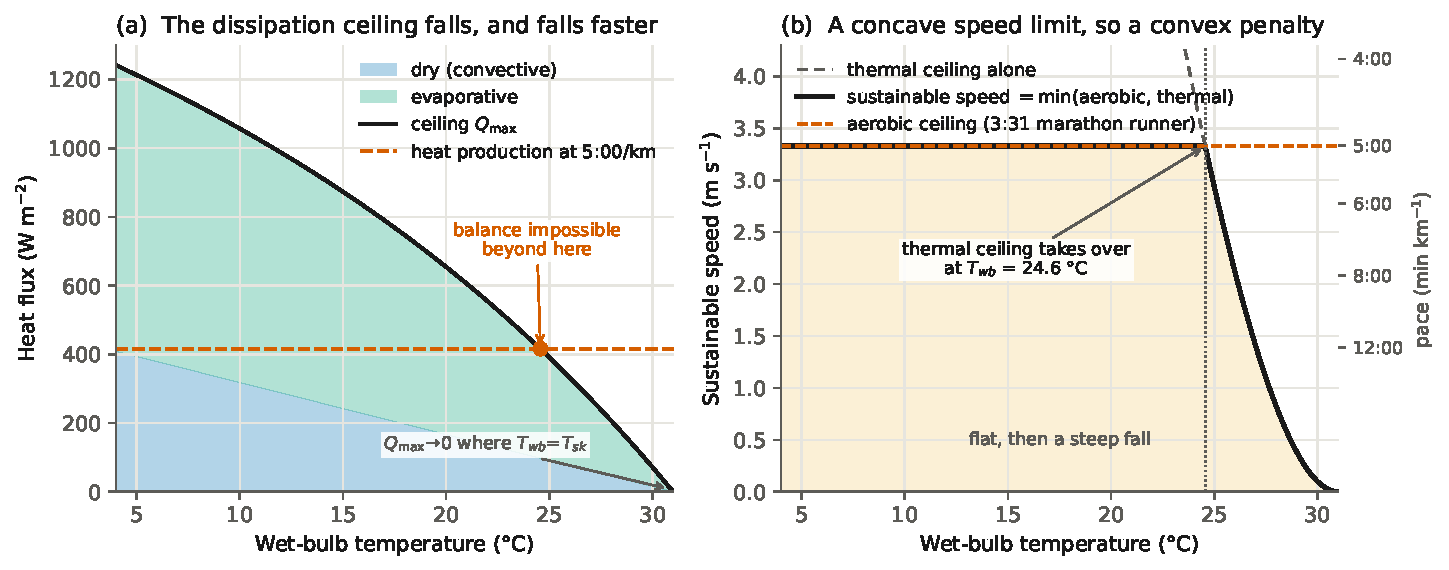
\includegraphics[width=\linewidth]{figures/fig_heat_ceiling.pdf}
  \caption{The heat balance read as a constraint on pace, for the reference
  runner. (a)~The dissipation ceiling $Q_{\max}$ against wet-bulb temperature,
  split into its dry and evaporative parts; the dashed line is the heat the
  runner produces at $5{:}00\,\mathrm{min\,km^{-1}}$. Where the two cross,
  steady-state balance at that pace is no longer available. On this axis the
  dry term never reverses sign, since wetted skin cannot be cooler than the
  wet-bulb temperature. (b)~The speed the balance permits, $v_{\max} \propto
  \Phi^2$, against the runner's own aerobic ceiling. The sustainable speed is
  the lower of the two, so it is flat while the aerobic limit binds and then
  falls steeply. Note that the thermal ceiling takes over only at
  $T_{wb} = 24.6\,^{\circ}$C, roughly WBGT $25$ to $29\,^{\circ}$C depending on
  humidity and solar load, which is far too warm to produce the breakpoint near
  $16\,^{\circ}$C that the learned curve shows; Section~\ref{app:physics:graded}
  takes up what does.}
  \label{fig:heat_ceiling}
\end{figure}

Table~\ref{tab:wbtradeoff} and Figure~\ref{fig:wetbulb_isopleth} walk one
wet-bulb isopleth. Every row sits at $T_{wb} = 22\,^{\circ}$C and is therefore
the same thermal environment by \eqref{eq:qmax-wb}, though assembled quite
differently: the first is a cool morning at $92\%$ humidity, the last desert
heat at $18\%$. As air temperature rises the dry route degrades from shedding
$121$ to \emph{gaining} $152\,\mathrm{W\,m^{-2}}$, reversing sign at
$31\,^{\circ}$C where air and skin are equal, while the drier air widens the
skin-to-air vapour-pressure gradient and evaporative capacity rises by exactly
as much. The trade is exact rather than approximate: along a line of constant
wet-bulb temperature $h_e\,\mathrm{d}P_a = -h_c\,\mathrm{d}T_a$ by definition,
so the two terms move by equal and opposite amounts and their sum cannot shift.
The heavy weight on the wet-bulb term in the definition of WBGT is therefore
recoverable from the heat balance rather than merely calibrated against
outcomes.

\begin{table}[!ht]
\centering\small
\caption{One wet-bulb isopleth, at $T_{wb} = 22\,^{\circ}$C for the reference
runner, with no solar load. Dry and evaporative capacity trade off exactly and
their sum $Q_{\max}$ does not move. The two right-hand columns show what that
invariance does \emph{not} cover: the strain the runner carries, and the fluid
it costs, both rise along the same line. Figure~\ref{fig:wetbulb_isopleth}
draws the same five conditions.}
\label{tab:wbtradeoff}
\begin{tabular}{@{}rrrrrrr@{}}
\toprule
 & & \multicolumn{3}{c}{Heat-loss capacity (W\,m$^{-2}$)}
   & \multicolumn{2}{c}{Cost to the runner} \\
\cmidrule(lr){3-5}\cmidrule(lr){6-7}
Air temp. & Rel.\ hum. & Dry & Evaporative & Total
   & Required & Sweat \\
(\textdegree C) & (\%) & $C$ & $E_{\max}$ & $Q_{\max}$
   & $w_{req}$ & (L\,h$^{-1}$) \\
\midrule
23 & 92 & $+121$ & 434 & 555 & 0.68 & 0.81 \\
29 & 54 & $+30$  & 525 & 555 & 0.74 & 1.06 \\
31 & 45 & $0$    & 555 & 555 & 0.75 & 1.14 \\
35 & 32 & $-61$  & 616 & 555 & 0.78 & 1.31 \\
41 & 18 & $-152$ & 707 & 555 & 0.80 & 1.56 \\
\bottomrule
\end{tabular}
\end{table}

\begin{figure}[!ht]
  \centering
  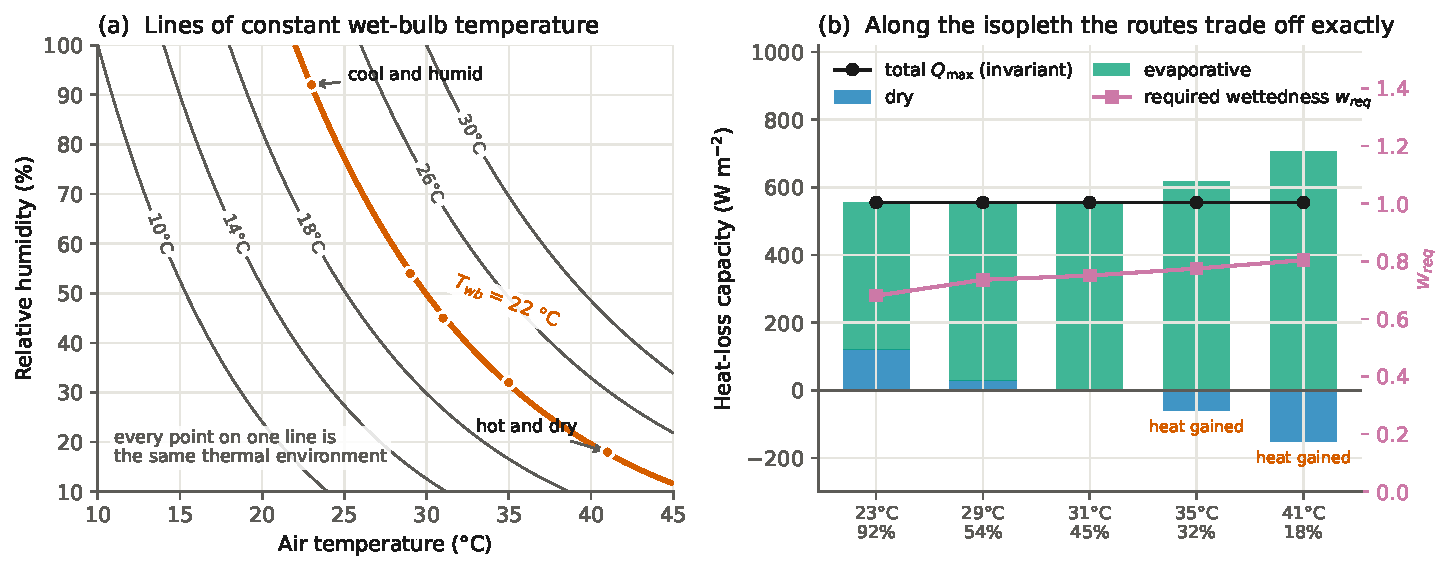
\includegraphics[width=\linewidth]{figures/fig_wetbulb_isopleth.pdf}
  \caption{What a wet-bulb temperature summarizes. (a)~Lines of constant
  $T_{wb}$ on the air-temperature and humidity plane. Any two points on one
  line present the runner with the same dissipation ceiling, which is why a
  single number can stand in for two. The highlighted line carries the five
  conditions of Table~\ref{tab:wbtradeoff}, from a cool humid morning to desert
  heat. (b)~Walking that line: the dry and evaporative routes trade off exactly,
  so their total does not move, but the required wettedness rises anyway. The
  invariance covers the ceiling, not the strain, which is one principled reason
  to expect a model conditioned on WBGT alone to leave residual variance.}
  \label{fig:wetbulb_isopleth}
\end{figure}

The invariance is narrower than it first appears, and the last two columns of
Table~\ref{tab:wbtradeoff} say how. Wet-bulb temperature is a sufficient
statistic for the dissipation \emph{ceiling}, exactly, but not for the
\emph{strain}. Because the runner is a heat source of fixed output, $E_{req} =
H_{prod} - C$ moves with the dry term, so $w_{req} = (H_{prod} - C)/(Q_{\max} -
C)$ is invariant only in the degenerate case $H_{prod} = Q_{\max}$. Along this
isopleth it climbs from $0.68$ to $0.80$, approaching ISO's unacclimatised
limit of $0.85$, while the sweat rate needed to hold pace nearly doubles from
$0.81$ to $1.56\,\mathrm{L\,h^{-1}}$. At matched wet-bulb, hot and dry is
therefore harder on a runner than cool and humid, because the dry route turning
from ally to adversary costs more than the widened vapour-pressure gradient
returns.

\subsection{A concave speed limit makes a convex penalty}
\label{app:physics:convex}

Combining \eqref{eq:pinned} and \eqref{eq:qmax-wb} gives the speed limit
explicitly. Because the transfer coefficients scale with the square root of
running speed, the balance $\kappa v = A\,h_c(v)\,\Phi$ solves in closed form,
\begin{equation}
  v_{\max}(T_{wb}) \;=\; \left(\frac{8.3\,A}{\kappa}\right)^{\!2}\Phi(T_{wb})^{2}
  \;=\; 0.0044\;\Phi(T_{wb})^{2}\ \mathrm{m\,s^{-1}} .
  \label{eq:vmax}
\end{equation}
The pace penalty relative to a cool reference is then
$v_{ref}/v_{\max} - 1$, which is proportional to $\Phi^{-2}$. Differentiating
twice, for any power $p > 0$,
\begin{equation}
  \frac{\mathrm{d}^2}{\mathrm{d}T_{wb}^2}\,\Phi^{-p}
  \;=\; p\,\Phi^{-p-2}\Bigl[(p+1)\,\Phi'^{\,2} \;-\; \Phi\,\Phi''\Bigr]
  \;>\; 0,
  \label{eq:convex-ceiling}
\end{equation}
in which both bracketed terms are positive, the first because it is a square
and the second because $\Phi > 0$ and $\Phi'' < 0$ by \eqref{eq:phi-derivs}.
The pace penalty implied by the ceiling is therefore strictly convex in
wet-bulb temperature. The result does not depend on the constants, on how the
transfer coefficients scale with speed (any $p$ will do, and $p=1$ is the
constant-coefficient case), or on the runner. It requires only that saturation
vapour pressure be increasing and convex, which is thermodynamics rather than
physiology.

Two features of \eqref{eq:vmax} are worth reading off directly.
Figure~\ref{fig:heat_ceiling}(b) draws it. First, the sustainable speed is the
lesser of this thermal limit and the runner's aerobic limit, so the predicted
shape is flat and then falling, which is the qualitative signature the learned
curve shows. Second, the fall has an asymptote rather than a slope: $v_{\max}$
reaches zero at $T_{wb} = T_{sk}$, because at that point the head is zero and
no heat leaves at all. For a runner whose skin sits at $31\,^{\circ}$C that
wall is at a wet-bulb temperature of $31\,^{\circ}$C. It is the running
counterpart of the wet-bulb limit discussed for resting humans
\citep{sherwood2010}, and it is lower for the same reason skin is cooler: running-speed airflow over wet skin holds
the surface below air temperature, and the wall follows the surface down. The
runner's own heat production then ends compensable racing some six degrees
below even that wall. This is why a convex response is the physically expected
one: the constraint does not saturate as conditions worsen, it tightens toward
a vertical asymptote.

Against that, one thing the ceiling argument cannot do is explain the flat band
in the measured curve. For the reference runner the thermal limit overtakes the
aerobic limit only at $T_{wb} = 24.6\,^{\circ}$C, which corresponds to WBGT
between about $25$ and $29\,^{\circ}$C depending on humidity and solar load, and
reading it through required wettedness instead puts the crossing at WBGT $25.7$
to $27.1\,^{\circ}$C depending on whether $w_{\max}$ is taken as ISO's
unacclimatised $0.85$ or an acclimatised $1.0$. Either route is some ten
degrees too warm to account for a breakpoint near $16\,^{\circ}$C. A runner who
held pace until the hard limit bound would show almost no penalty and then a
collapse, which resembles no measured curve. The hard ceiling supplies the
shape of the response but not its onset.

\subsection{Below the ceiling, the same curvature acts on a graded strain}
\label{app:physics:graded}

Runners evidently concede pace long before balance becomes impossible, so the
operative quantity is a graded measure of strain rather than a threshold.
Thermal compensability supplies one. It is $w_{req} = E_{req}/E_{\max}$, where
$E_{req} = H_{prod} - (C + R)$ is the evaporation needed for balance and
$E_{\max}$ the maximum the environment will accept \citep{taylor2006,
belding1955}. Because evaporation scales with wetted area, $w_{req}$ is also
the fraction of the skin that must be covered in sweat, which is what makes it
a graded measure of strain rather than a bare ratio.

Its convexity is the same fact in different clothing, and it is worth being
explicit that this is a corollary rather than an independent finding. The
numerator rises exactly linearly in air temperature, since dry exchange is
proportional to the skin-to-air gradient and simply reverses sign once air
passes skin temperature. The denominator falls at an accelerating rate, for the
one reason given in \eqref{eq:phi-derivs}. Writing $w_{req} = N/D$ with $N$
affine and increasing and $D$ positive, decreasing and concave,
\begin{equation}
  w_{req}'' \;=\; \frac{-\,N D'' D \;-\; 2 N' D' D \;+\; 2 N D'^{2}}{D^{3}},
  \label{eq:convex}
\end{equation}
in which all three numerator terms are positive, since $D'' < 0$, $N' > 0$ and
$D' < 0$. Convexity is therefore a property of the heat balance and not an
artifact of the constants chosen. It is stated here on the air-temperature axis;
because wet-bulb globe temperature is very nearly affine in wet-bulb temperature
over the range plotted---its slope moves only from $1.047$ to $1.042$ across
$10$ to $38\,^{\circ}$C of air temperature---the property carries over to the
axis of Figure~\ref{fig:heat_cost}, which we confirm numerically at relative
humidities from 30 to 90\%.

A proportional response to $w_{req}$ still does not quite describe the measured
curve. Rescaled to match the learned penalty at its endpoints, $w_{req}$
predicts a $0.9\%$ slowdown at $16\,^{\circ}$C WBGT where the learned curve
shows $0.3\%$: strain rises perceptibly in the cool range while measured pace
does not. What reconciles them is a single convex map from strain to conceded
pace. Fitting $\text{penalty} = c\,w_{req}^{\,k}$ over the $16$ to
$28\,^{\circ}$C range returns $k \approx 1.9$, and that one exponent does both
jobs at once: it suppresses the response at low strain, producing the flat band
without a threshold, and it steepens the response at high strain.

The exponent is fitted rather than derived, but it is not unconstrained, and the
bound is the more useful statement. Consider the two natural candidates for what
a runner concedes pace in proportion to. If it is thermal strain itself, the
penalty tracks $w_{req}$, and the predicted steepening over the two bands used
below is $1.80$. If instead it is the fluid cost of sustaining that strain, the
governing quantity is the sweat that must be \emph{produced} rather than the
sweat that evaporates, $w_{req}/\eta_{sw}$, since sweat beyond the evaporative
ceiling drips rather than cools \citep{taylor2006}. Sweating efficiency
$\eta_{sw}$ is itself a measured function of wettedness, falling at fully wetted
skin to $0.50$ under ISO 7933, whose curve follows the working measurements of
\citet{alber1985}, and to $0.67$ under the resting measurements of
\citet{candas1979}; both forms give a predicted steepening near $5$. The
observed $2.18$ lies between the two and nearer the strain end, so runners
appear to concede pace largely in proportion to thermal strain, with a secondary
sensitivity to fluid cost as the skin approaches saturation. Both bounds come
from measured physiology rather than from a free parameter, but a bracket is not
a derivation, and one caveat attaches at the hot end: $w_{req}$ exceeds unity at
$28\,^{\circ}$C for this runner, so both efficiency relations are there being
read beyond the range over which they were established.

\subsection{The same balance, read as a demand on the circulation}
\label{app:physics:circulation}

Nothing above says how heat reaches the skin, and the answer supplies both a
second constraint and a check on the first. Heat is generated in working muscle
and lost at the surface, and the only transport of consequence between them is
convection by blood. That imposes a second balance alongside
\eqref{eq:pinned}: the skin blood flow $\dot{Q}_{sk}$ must carry the whole
production across the core-to-skin temperature gradient,
\begin{equation}
  H \;=\; \rho c_b\,\dot{Q}_{sk}\,\bigl(T_{core} - T_{sk}\bigr)
  \qquad\Longrightarrow\qquad
  \dot{Q}_{sk} \;=\; \frac{H}{\rho c_b\,(T_{core} - T_{sk})},
  \label{eq:skbf}
\end{equation}
with $\rho c_b \approx 3.8\,\mathrm{kJ\,L^{-1}\,K^{-1}}$ the volumetric heat
capacity of blood.\footnote{Published values used in this calculation span
$3.64$ to $4.19\,\mathrm{kJ\,L^{-1}\,K^{-1}}$, the upper end being models that
treat blood as water. The spread does not affect the shape of the result, only
its level.} For the reference runner holding a core temperature of
$39\,^{\circ}$C, this requires at least $1.5\,\mathrm{L\,min^{-1}}$ to the skin
when skin sits at $31\,^{\circ}$C, and at least $3.1$ when it sits at
$35\,^{\circ}$C. \citet{cheuvront2010} run the same calculation for a
world-class marathoner and tabulate the same accelerating pattern, $1.1$,
$2.2$ and $4.4\,\mathrm{L\,min^{-1}}$ as the core-to-skin gradient closes from
$8$ to $4$ to $2\,^{\circ}$C.

These are lower bounds. They credit the skin with the whole production, which
overstates it by the small respiratory share, but they also assume blood
returns from the skin fully cooled to skin temperature, which countercurrent
exchange prevents and which understates the requirement by a good deal more.
The margin is real but not large: cutaneous flow reaches roughly $6$ to
$8\,\mathrm{L\,min^{-1}}$ at rest and plateaus near half of that maximum during
exercise, against a cardiac output that in trained men at exhaustion in the
heat runs near $20\,\mathrm{L\,min^{-1}}$.

Two things follow. The first is the competition the main text refers to. Cardiac
output is finite, and blood directed to the cutaneous beds for cooling is not
available to working muscle, nor does it all return promptly, so a rising
cutaneous demand shows up as some combination of reduced muscle perfusion,
reduced stroke volume with a compensating heart rate, and a compressed
$\dot{V}\mathrm{O}_2$max reserve at unchanged pace. This is the axis
\citet{cheuvront2010} identify, and it is why the strain arrives as
cardiovascular before it arrives as thermal.

The second is structural, and it matters for how the competing accounts in
Section~\ref{app:physics:limits} should be read. The right-hand side of
\eqref{eq:skbf} is a reciprocal of the core-to-skin gradient, so it is convex in
skin temperature for the same elementary reason that $\Phi^{-p}$ is convex in
\eqref{eq:convex-ceiling}: the demand does not rise steadily as the gradient
closes, it accelerates, and it diverges as skin temperature approaches core
temperature. The cardiovascular route therefore carries the same curvature as
the evaporative one, and it must, because the two are consecutive links in one
chain rather than rival mechanisms. Heat that cannot leave the skin raises skin
temperature, which narrows the gradient, which raises the flow required to
deliver the next joule. A convex response is what a chain of this shape
produces regardless of which link is measured, which is a reason to hold the
convexity finding more confidently than any particular mechanism attributed to
it.

\subsection{Why duration matters}
\label{app:physics:duration}

Everything so far has assumed balance. It need not hold instantaneously, since
heat can be stored as a rise in core temperature, and a runner may therefore
hold a pace the environment will not support --- for a while. What that buys is
finite, and pricing it exactly is what separates a marathon from a mile. Taking
tissue heat capacity as $3474\,\mathrm{J\,kg^{-1}\,K^{-1}}$
\citep{burton1935},\footnote{Burton adopted $0.83\,\mathrm{kcal\,kg^{-1}}$ per
degree ``by general custom'' and bounded it only to $0.7$--$0.9$, so the figure
carries perhaps ten percent of slack. The widely quoted $3500$ has no primary
source, and a recent direct measurement of tissue puts it some seventeen
percent lower still. None of this matters here: the storage term is small at
the distance we model, and the argument is that it is small.} the
$2.5\,^{\circ}$C rise a runner will spend in a $70\,\mathrm{kg}$ body is
\begin{equation}
  B \;=\; m\,c\,\Delta T_{core} \;\approx\; 608\,\mathrm{kJ},
  \label{eq:bank}
\end{equation}
a fixed quantity of heat, spent once and not replaced during the race.

The rate at which it is spent is set by the same strain measure as before. Once
$w_{req}$ passes unity the skin cannot get any wetter, so evaporation saturates
at $E_{\max}$ and every further joule is stored:
\begin{equation}
  S \;=\; E_{req} - E_{\max} \;=\; E_{\max}\,\bigl(w_{req} - 1\bigr).
  \label{eq:storage}
\end{equation}
Core temperature then climbs at $S/mc$ and the allowance is exhausted after
$t^{*} = B/S$. Table~\ref{tab:duration} and Figure~\ref{fig:duration_bank}(a)
evaluate this for the reference runner holding
$5{:}00\,\mathrm{min\,km^{-1}}$, and the striking feature is how sharply the
ladder steepens. At $w_{req} = 1.05$ core temperature rises at
$0.6\,^{\circ}\mathrm{C\,h^{-1}}$ and the runner reaches the finish before the
allowance does, so a five percent overshoot is, for practical purposes, free. At
$1.10$ it is spent at $26\,\mathrm{km}$, which is a race that goes wrong late
and not gradually; at $1.25$ at $11\,\mathrm{km}$; at $1.50$ before
$7\,\mathrm{km}$. Nothing in that ladder is a threshold. It is one hyperbola,
$t^{*} \propto (w_{req}-1)^{-1}$, and the flat measured response at cool
temperatures and the steep one at warm are its two ends.

\begin{table}[!ht]
\centering\small
\caption{What the storage allowance of \eqref{eq:bank} buys, for the reference
runner holding $5{:}00\,\mathrm{min\,km^{-1}}$ in air at $60\%$ relative
humidity under $200\,\mathrm{W\,m^{-2}}$ of solar load. Each row is the
environment that puts the runner at that required wettedness. The last row is
the limit in which the environment carries nothing away at all, and its
distance is $d_{bank}$ of \eqref{eq:dbank} --- the floor no runner gets below,
whatever the weather. Figure~\ref{fig:duration_bank} draws both halves.}
\label{tab:duration}
\begin{tabular}{@{}rrrrr@{}}
\toprule
Required & WBGT & Stored & Core rise & Allowance \\
wettedness & (\textdegree C) & $S$ (W) & (\textdegree C\,h$^{-1}$)
   & spent at \\
\midrule
1.05 & 27.5 & 40  & 0.6  & 50.5\,km \\
1.10 & 27.9 & 78  & 1.1  & 26.1\,km \\
1.25 & 28.9 & 177 & 2.6  & 11.5\,km \\
1.50 & 30.1 & 307 & 4.5  & 6.6\,km \\
\midrule
\multicolumn{2}{@{}l}{no dissipation at all} & 770 & 11.4 & 2.6\,km \\
\bottomrule
\end{tabular}
\end{table}

That last row generalises, and it is the cleanest statement in this section.
Suppose the environment carries nothing away, so the whole of production is
stored. The allowance then lasts $B/H$ seconds, and over that time the runner
covers
\begin{equation}
  d_{bank} \;=\; v\,\frac{B}{\kappa\,v} \;=\; \frac{B}{\kappa}
  \;=\; \frac{c\,\Delta T_{core}}{c_{run}} \;\approx\; 2.6\,\mathrm{km}.
  \label{eq:dbank}
\end{equation}
Speed cancels, because production and distance both scale with it. Body mass
cancels too, because the allowance and the cost of covering ground both scale
with that, leaving running economy carried as heat per kilogram per metre,
$c_{run} = \kappa/m \approx 3.3\,\mathrm{J\,kg^{-1}\,m^{-1}}$. What is left is
a distance fixed by three quantities --- tissue heat capacity, the
core-temperature rise the runner is willing to spend, and economy --- and by
nothing whatever about the weather, since the derivation never consulted it. Out to roughly two and a half kilometres, a runner could shed no
heat whatsoever and still finish inside the tolerable rise. Heat cannot bind a
race shorter than that, in any conditions, at any pace, for anybody.

The same cancellation gives the general version. Over a race of distance $d$
the allowance is worth $B/(\kappa d) = d_{bank}/d$ of the runner's total heat
production, again independently of pace and of body mass, which is the curve of
Figure~\ref{fig:duration_bank}(b). It is worth twenty-six times production over
$100\,\mathrm{m}$, $1.75$ times over $1500\,\mathrm{m}$, $88\%$ over
$3000\,\mathrm{m}$, half over $5000\,\mathrm{m}$, a quarter over
$10\,\mathrm{km}$, an eighth over the half marathon and $6\%$ over the marathon.
Read as a fraction of the problem, heat is a rounding error at sprint distances,
a real but secondary term through the middle distances, and essentially the
whole of the problem at the marathon. This is a prediction about where the
constraint switches on, and it is worth noting that it lands on distance rather
than on time.

\begin{figure}[!ht]
  \centering
  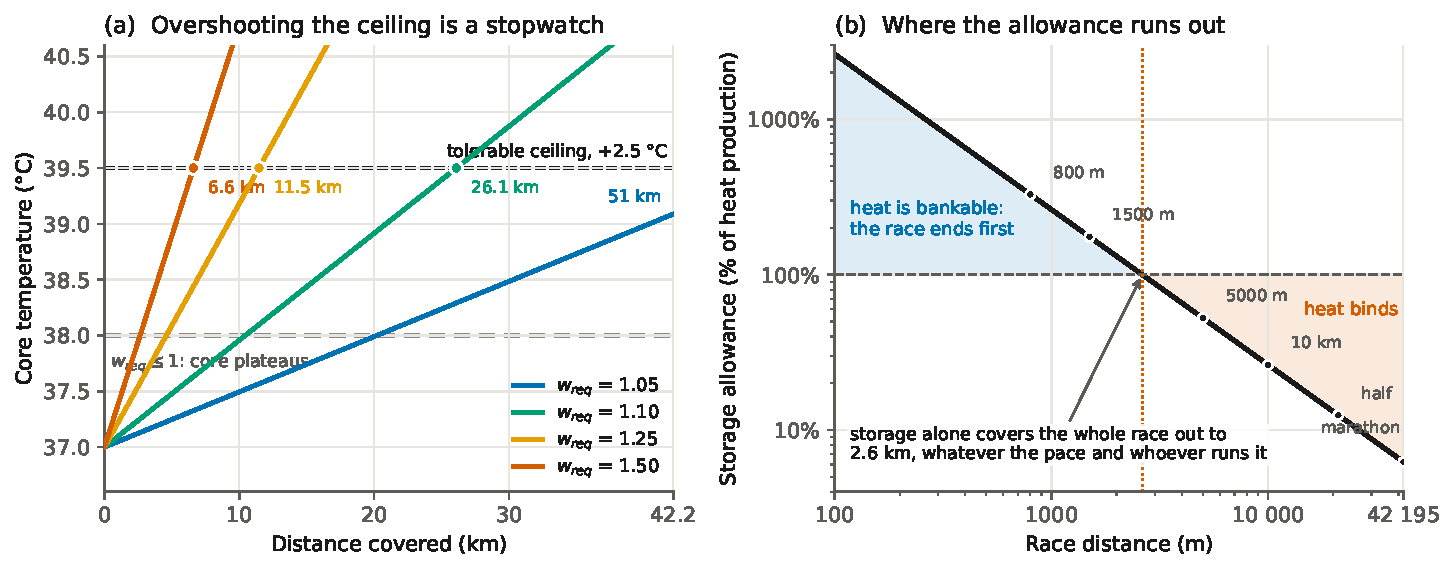
\includegraphics[width=\linewidth]{figures/fig_duration_bank.pdf}
  \caption{Why the same physics governs a marathon and spares a mile.
  (a)~Core temperature against distance covered, for the reference runner
  holding $5{:}00\,\mathrm{min\,km^{-1}}$ at four required wettednesses
  (Table~\ref{tab:duration}); the dot marks where the $2.5\,^{\circ}$C
  allowance is spent and the runner must slow. Below $w_{req} = 1$ balance
  closes and core temperature plateaus instead, so the trajectory never
  arrives. Lines are straight because mean skin temperature is held fixed,
  which makes them optimistic: as the surface balance fails, skin warms, the
  core-to-skin gradient closes and the real trajectory bends upward
  (Section~\ref{app:physics:circulation}). (b)~The allowance as a share of the
  runner's total heat production against race distance. The share is exactly
  $d_{bank}/d$, so the curve is the same for every runner and every pace, and
  it crosses unity at $2.6\,\mathrm{km}$: shorter than that, storage alone
  could absorb the entire race.}
  \label{fig:duration_bank}
\end{figure}

The empirical pattern agrees. \citet{guy2014} report faster sprint performances
in the heat alongside slower marathons. The two halves of that finding are not
in tension: at $100\,\mathrm{m}$ the allowance is twenty-six times production,
so \eqref{eq:dbank} says heat imposes no constraint at all there, which leaves
the ergogenic effect of warmer muscle --- outside this balance, and not
predicted by it --- free to dominate. What the balance does predict is the
distance at which that freedom ends. \citet{leslie2024} find
critical velocity falling $3.7\%$ and then a further $2.9\%$ across heat indices
of $20$, $38$ and $55\,^{\circ}$C --- a \emph{decelerating} response, and the
only regime in this appendix where we predict one, since critical velocity is a
three-to-thirty-minute construct and therefore sits astride $d_{bank}$ where
the storage term still covers most of the imbalance. The same reasoning gives a
reason beyond exposure time why identical conditions cost a slower finisher
more: the allowance is a fixed quantity of heat, so spreading it over a longer
race dilutes it in exactly the proportion $d_{bank}/d$. \citet{taylor2006} list
duration of competition among the determinants of compensability for the same
reason.

Two caveats attach to the trajectories rather than to the accounting. The first
is that the $2.5\,^{\circ}$C allowance is a modelling convention rather than a
measured constant. The rise a runner will accept differs between individuals
and shifts with acclimatisation \citep{periard2015}, and \eqref{eq:dbank} is
exactly proportional to it, so $d_{bank}$ inherits that softness without
attenuation: it is a scale, not a threshold. The second is that holding mean
skin temperature fixed makes
the straight lines of Figure~\ref{fig:duration_bank}(a) the best case. In a
failing balance the skin warms, which narrows the core-to-skin gradient and
raises the blood flow required to move the next joule
(Section~\ref{app:physics:circulation}), so the real trajectory accelerates and
the distances in Table~\ref{tab:duration} are upper bounds. Both caveats push
the same way, which is toward heat binding sooner than tabulated, not later.

\subsection{Does it predict the curvature we measured?}
\label{app:physics:curvature}

Between the $20$--$24$ and $24$--$28\,^{\circ}$C WBGT bands the learned curve of
Section~\ref{sec:results} steepens by a factor of $2.18$. Evaluated over the
same bands, $w_{req}$ alone steepens by $1.80$, and across relative humidities
of $40$--$85\%$ and solar loads of $0$--$500\,\mathrm{W\,m^{-2}}$ the predicted
factor spans $1.5$ to $2.7$. The prediction brackets the observation, and the
direction of any residual gap is the expected one: with a convex strain-to-pace
map the heat balance supplies a lower bound on curvature, not an equality.

The prediction is robust to most of its inputs and fragile in one. Varying the
convective coefficient across the full published span at this speed, $10.4$ to
$33.7\,\mathrm{W\,m^{-2}\,K^{-1}}$, moves the predicted factor only to
$1.4$--$2.8$; varying metabolic rate from a $60\,\mathrm{kg}$ runner at
$5{:}00\,\mathrm{min\,km^{-1}}$ to a $70\,\mathrm{kg}$ runner at $4{:}00$ moves
it to $1.5$--$2.8$. Mean skin temperature dominates instead. At the
laboratory-running value of $35\,^{\circ}$C the prediction falls to $1.3$--$1.8$
and misses the observation; at $29\,^{\circ}$C it widens to $1.6$--$4.3$. We
adopt $31\,^{\circ}$C because \citet{aylwin2023} measured mean skin temperature
falling from $29.8$ to $28.9\,^{\circ}$C through the men's marathon at the 2019
World Championships, below air temperature and well below laboratory treadmill
values, with running-speed airflow over wet skin the reason.

That measurement carries a caveat which cuts against us and is worth stating.
Aylwin's thermography covers exposed skin, some $64\%$ of body surface area,
while the heat balance wants a whole-body mean that includes covered skin, which
runs warmer. Weighting the covered remainder at anything from $32$ to
$38\,^{\circ}$C puts the whole-body mean between $30.3$ and $32.5\,^{\circ}$C,
over which range the predicted factor spans $1.4$ to $3.1$ and continues to
bracket the observation; the prediction fails only above about
$33\,^{\circ}$C, which no plausible weighting of these measurements reaches. The
agreement is therefore correct in sign and order of magnitude but not sharp, and
the width of the band is dominated by a quantity the corpus does not observe.

\subsection{Does the penalty survive on the thermometer's axis?}
\label{app:physics:drybulb}

Everything so far is stated on a humidity-weighted axis, which invites the
objection that the finding is a property of the index rather than of the
weather. It is not, and separating the two yields the sharpest prediction in
this appendix.

Hold relative humidity fixed and vary air temperature. The head becomes
$\Phi(T_a) = (T_{sk} - T_a) + \mathrm{LR}\,(P_s(T_{sk}) - \mathrm{RH}\cdot
P_s(T_a))$, so
\begin{equation}
  \Phi''(T_a) \;=\; -\,\mathrm{LR}\cdot\mathrm{RH}\cdot P_s''(T_a).
  \label{eq:phi-rh}
\end{equation}
The curvature is not merely humidity-sensitive; it is exactly proportional to
relative humidity, and it vanishes identically in perfectly dry air. The
consequence for the graded measure is stark and is drawn in
Figure~\ref{fig:drybulb_axis}(a): $w_{req}$ is a strictly convex function of air
temperature at every humidity we can race in, and an exactly linear one at
$\mathrm{RH} = 0$, where its denominator stops depending on air temperature
altogether. All of the acceleration in the strain measure is a humidity effect
wearing a temperature label.

The two measures part company here, which makes the dry end a discriminating
test rather than a curiosity. The ceiling penalty retains a residual convexity
even in dry air, because a reciprocal of an affine function is still convex, so
it predicts a mild bend where $w_{req}$ predicts none: at $25\,^{\circ}$C and
zero humidity the penalty's second derivative is $1.6\times10^{-4}$ against
$5.3\times10^{-3}$ at $50\%$ and $7.3\times10^{-2}$ at $90\%$. A corpus with
enough genuinely hot and dry racing would separate the two accounts. Ours does
not contain it.

Finally, the practical question. Because the model was shown wet-bulb globe
temperature and nothing else, it cannot be asked directly what an extra degree
of dry-bulb heat costs; but the learned curve can be composed with the map from
$(T_a, \mathrm{RH})$ to WBGT and read on the thermometer's axis, which is
Figure~\ref{fig:drybulb_axis}(b) and Table~\ref{tab:drybulb}. The slowdown does
not depend on the index for its existence. At $50\%$ humidity and a solar load
of $200\,\mathrm{W\,m^{-2}}$, warming from $10$ to $25\,^{\circ}$C of air
temperature costs $1.7\%$ of pace, and warming to $30\,^{\circ}$C costs $3.7\%$;
the same $25\,^{\circ}$C day costs $1.0\%$ at $30\%$ humidity and $3.5\%$ at
$90\%$. The penalty rises monotonically along every constant-humidity line, and
it accelerates along each of them, so the shape reported in
Section~\ref{sec:results} is a property of the weather rather than of the
weighting. What the composition also shows is how much the thermometer alone
conceals: a single air temperature spans a threefold range of cost depending on
the humidity attached to it, which is the practical case for carrying the
composite index rather than the raw reading.

\begin{figure}[!ht]
  \centering
  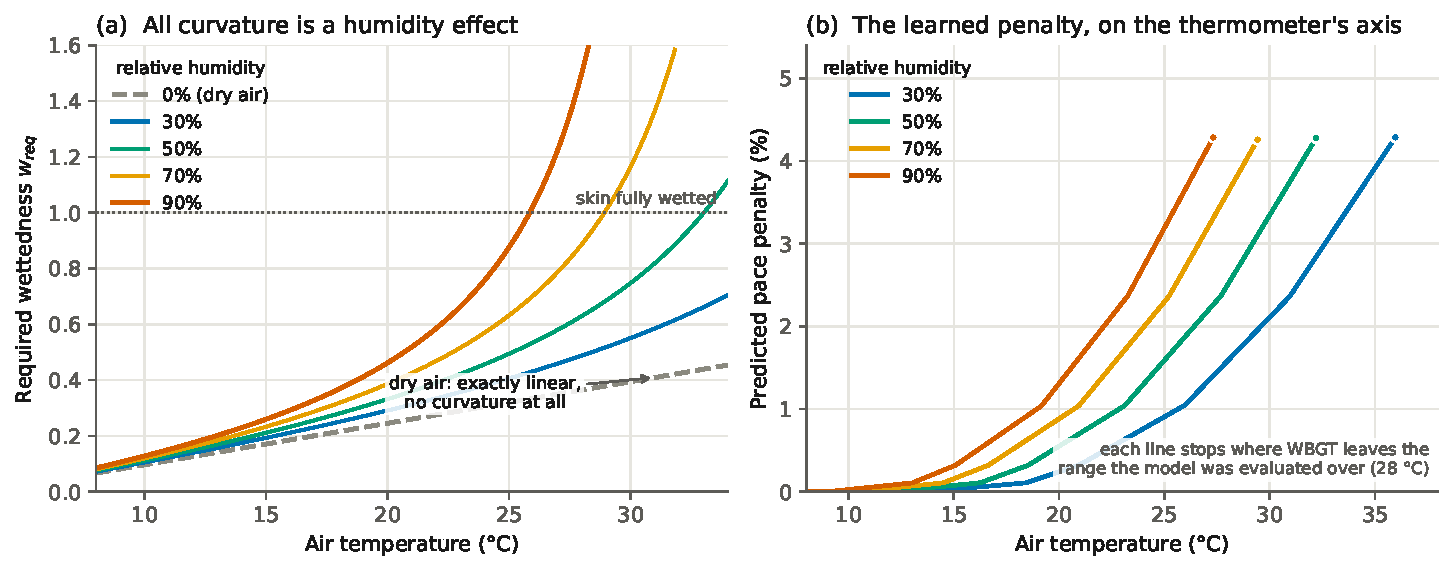
\includegraphics[width=\linewidth]{figures/fig_drybulb_axis.pdf}
  \caption{The response on the dry-bulb axis, at fixed relative humidity.
  (a)~Required wettedness against air temperature. The curvature is exactly
  proportional to humidity by \eqref{eq:phi-rh}, so the dry-air case is a
  straight line and every other case bends; the acceleration in the strain
  measure is entirely a humidity effect. (b)~The learned population curve of
  Figure~\ref{fig:heat_cost} composed with the map from air temperature and
  humidity to WBGT, at a solar load of $200\,\mathrm{W\,m^{-2}}$ and
  $1\,\mathrm{m\,s^{-1}}$ of wind. Each line stops where WBGT leaves the range
  over which the model was evaluated. Drawn by linear interpolation of the
  anchor values reported in Section~\ref{sec:results}, which is the source of
  the visible kinks.}
  \label{fig:drybulb_axis}
\end{figure}

\begin{table}[!ht]
\centering\small
\caption{The learned penalty re-expressed on the dry-bulb axis: percent pace
slowdown relative to $10\,^{\circ}$C of air temperature at the same humidity,
with a solar load of $200\,\mathrm{W\,m^{-2}}$ and $1\,\mathrm{m\,s^{-1}}$ of
wind. Dashes mark conditions whose WBGT exceeds $28\,^{\circ}$C, beyond the
range the model was evaluated over. Reading across a row isolates the cost of
humidity at fixed temperature; reading down a column isolates the cost of
temperature at fixed humidity.}
\label{tab:drybulb}
\begin{tabular}{@{}rrrrr@{}}
\toprule
Air temp. & \multicolumn{4}{c}{Relative humidity} \\
\cmidrule(lr){2-5}
(\textdegree C) & 30\% & 50\% & 70\% & 90\% \\
\midrule
10 & 0.00 & 0.00 & 0.00 & 0.03 \\
15 & 0.03 & 0.10 & 0.18 & 0.29 \\
20 & 0.24 & 0.59 & 1.00 & 1.45 \\
25 & 1.03 & 1.70 & 2.34 & 3.53 \\
30 & 2.17 & 3.74 & --- & --- \\
\bottomrule
\end{tabular}
\end{table}

\subsection{What this does and does not establish}
\label{app:physics:limits}

The argument constrains shape, not magnitude: nothing here derives the $5.0\%$
penalty of Section~\ref{sec:results}. What it does establish is narrower and
more durable. Convexity in the response is a theorem about the heat balance
rather than a feature fitted to the data, it holds on the ceiling and on the
graded strain measure alike, it survives the change of axis from wet-bulb to
WBGT and to dry-bulb at fixed humidity, and it traces in every case to one
term, $P_s''$. A linear penalty is not a simplification of this physics; it is
inconsistent with it.

Two competing explanations for the same curvature deserve naming, since neither
is excluded by our data. \citet{cheuvront2010} attribute an exponential decline
in aerobic performance to the cardiovascular axis; as
Section~\ref{app:physics:circulation} argues, that account shares the structure rather than
competing with it, but the two make different predictions about which
intervention helps and cannot be separated here. \citet{wang2024} attribute more
than half the marathon heat effect to reduced atmospheric oxygen partial
density, since warm air expands and rising vapour pressure displaces oxygen, a
mechanism that also scales with vapour pressure and therefore mimics the
humidity signature of the evaporative account while fitting a
piecewise-\emph{linear} form. Distinguishing the three requires measurements
this corpus does not contain.

A statistical objection applies to any pooled curve. Because the penalty is
strongly ability-dependent \citep{ely2007}, differential slopes combined with
differential field composition across warm and cool races can bend an aggregate
curve while no individual curve is convex. Our design is partly protected: the
curve of Section~\ref{sec:results} is the median of \emph{per-runner}
counterfactual sweeps, in which each runner's own response is traced with every
other channel held fixed, rather than a regression pooled across runners and
races. It is not protected against the possibility that the deep model has
learned one population-average response and applies it uniformly.

Finally, the critical wet-bulb temperature at running metabolic rates appears
not to have been measured. \citet{wolf2021} report critical WBGT falling from
$35.3\,^{\circ}$C at rest to $31.6\,^{\circ}$C at $30\%$
$\dot{V}\mathrm{O}_2$max, about $163\,\mathrm{W\,m^{-2}}$, while a marathon runs
above $400\,\mathrm{W\,m^{-2}}$. Occupational limit curves extrapolated that far
give $22\,^{\circ}$C WBGT (ACGIH) or $18\,^{\circ}$C (NIOSH), far below
conditions marathons are routinely held in, which suggests those curves do not
transfer to self-paced athletic work. Equation~\eqref{eq:vmax} makes the same
point from the other direction: it places an absolute wall at $T_{wb} = T_{sk}$
and, for the reference runner, an end to compensable racing some six degrees
below it. Neither number has been measured in runners. The gap is worth naming
as a target for measurement rather than filled by extrapolation here.

The calculations in this appendix are reproduced by
\texttt{verify\_heat\_convexity.py}, which is self-checking and prints a pass or
fail line for every number quoted above; the figures are built by
\texttt{build\_compensability\_figures.py}.
